
\chapter{Theoretical background}\label{chap:theory}

\section{FEST-Swing}\label{sec:fest-swing}

FEST (Fixtures for Easy Software Testing) is a collection of libraries whose mission is to simplify software testing. It is composed of various modules, which can be used with TestNG or JUnit. The most significant module is the FEST-Swing module.

The Swing module provides a simple and intuitive API for functional testing of Swing user interfaces, resulting in tests that are compact, easy to write, and read like a specification. Tests written using FEST-Swing are also robust. FEST simulates actual user gestures at the operating system level, ensuring that the application will behave correctly in front of the user. It also provides a reliable mechanism for GUI component lookup that ensures that changes in the GUI's layout or look-and-feel will not break the tests \cite{FESTMain}.

\subsection{Introduction}

A FEST-Swing test is testing either individual frames (the building blocks of a UI), or entire Swing applications or Applets. FEST simulates actual user gestures (mouse movements, keys presses) at the operating system level, ensuring that during the application will behave in the same way as in the front of the user. It uses AWT Robot, which generates events in the platform's native input queue. Thus, the test needs to create the components and make them visible on the screen, and the tests will actually moves the mouse cursor, and not just only generates mouse move events.

\subsection{Architecture}

FEST Swing's component fixture architecture is separated into several layers (from bottom to top):
\begin{enumerate}
\item BasicRobot: Simulates a user interacting with a mouse and keyboard. It uses the AWT Robot to generate native input events.
\item Component driver: This layer does all the ``heavy lifting.'' All interaction with a GUI component is done in this layer. It knows how to simulate events and check the state of a specific GUI component. For example, JComboBoxDriver knows how to simulate a user using a JComboBox (selecting a particular element) and how to verify the state of it (which element should be selected.)
\item Component fixture: This layer sits on top of the driver. It provides a fluent interface to that and makes the API easier to write and read. Users of FEST write their GUI tests using fixtures, not drivers. There is one fixture per Swing component, and each fixture has the same name as the Swing component they can handle ending with ``Fixture.'' For example, a JButtonFixture knows how to simulate user interaction and verify state of a JButton. Fixtures can be considered the ``user interface'' of the FEST-Swing library.
\end{enumerate}

The architecture also supports extensions, so developers of application using custom Swing components can write their own fixtures and component drivers.

\subsection{Example}

Writers of GUI tests need to use the fixtures located in the package org.fest.swing.fixture. These fixtures provide specific methods to simulate user interaction with a GUI component and they provide assertion methods that verify the state of the GUI component. Although it is possible to work with the FEST BasicRobot directly, the BasicRobot is too low-level and requires considerably more code than the fixtures.

As a concrete example, let us consider a very simple JFrame that contains a JTextField, a JLabel and a JButton, and component has its unique name. The expected behavior of this GUI is the following: when user clicks on the JButton, the text of the JTextField should be copied to the JLabel. (Figure \ref{fig:example_jframe}) 

\begin{figure}[h!] \label{fig:example_jframe}  
  \centering
    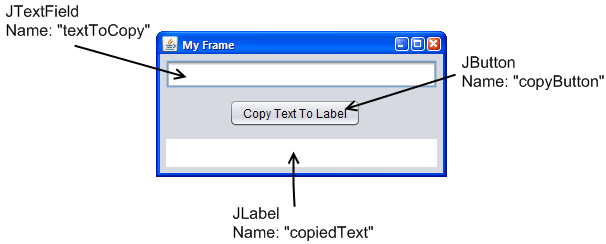
\includegraphics[width=0.6\textwidth]{images/example_jframe.png}
  \caption{A very simple JFrame that contains a JTextField, a JLabel and a JButton.}
\end{figure}

To the frame, the test's setup method needs to create the frame (in the EDT, delegating it with GuiActionRunner), create a fixture for it, and make it visible (Figure \ref{fig:example_setup_method}).

\begin{figure}[h!] \label{fig:example_setup_method}
\begin{lstlisting}
protected def onSetUp() : Unit = {
    val frame : MyFrame = GuiActionRunner.execute(new GuiQuery[MyFrame] {
        protected def executeInEDT() : MyFrame = new MyFrame
    })
    window = new FrameFixture(robot, frame)
    window.show() // shows the frame to test
}
\end{lstlisting}
\caption{The setup method creating the frame and the fixture, and making it visible.}
\end{figure}

The test method can use the fixture to simulate a user interacting with a GUI in order to verify that such GUI behaves as we expect. The user interactions and the assertions in the test are fluent and simple. The method looks up the UI components by their unique names. (Figure \ref{fig:example_test_method})

\begin{figure}[h!] \label{fig:example_test_method}
\begin{lstlisting}
@Test 
def shouldCopyTextInLabelWhenClickingButton : Unit = {
    window.textBox("textToCopy").enterText("Some random text")
    window.button("copyButton").click()
    window.label("copiedText").requireText("Some random text")
}
\end{lstlisting}
\caption{The test method.}
\end{figure}

It is important to mention that besides testing individual components that build up an application, FEST-Swing also supports testing entire applications. In such cases, the first tests starts up the application with ApplicationLauncher that understands how to launch an application using its main method. Once the application is started, the test just needs to find the application's main window.

\subsection{Threading model}

The documentation of FEST-Swing strongly advises to respect Swing's threading rules \cite{OracleSwingThreading} both in the tests and in the tested application (this remains only an advice because Swing itself does not enforce thread safety). In short, the cardinal rule is the following: creation and access (both read and write) of Swing components should be done in the Event Dispatch Thread (EDT.) Since JUnit and TestNG tests do not run on the EDT, creation and any direct access in the tests to Swing components should be delegated to EDT via the utility class GuiActionRunner (or via other tools).

To ensure that the threading rules are respected throughout the tests and the tested application, FEST Swing provides the class FailOnThreadViolationRepaintManager. It forces a test failure if access to Swing components is not performed on the EDT. However, it only detects component creation and writing, and is unable to detect read operations (component creation and writing triggers repaint events, but read does not).

\subsection{Limitations}\label{sec:fest-swing-limitations}

Because FEST-Swing is actually simulating user interaction, it needs an environment very similar to actual user environments: the tested application needs to be active and in focus, and needs to move the mouse. Therefore, that machine that the tests run on cannot be used for the entire duration of the tests. In addition, the tests probably fail whenever another applications unexpectedly gets the focus and covers the application's window (the mouse no longer clicks the correct application). This can become a burden because UI tests, by their nature, can take a significant amount of time to execute and especially when using agile development methods, it is preferable to run them frequently.

Because of this, it is common to delegate the tests to Continuous Integration (CI) systems (e.g. Hudson/Jenkins, TeamCity etc.) When the CI platform is based Linux, BSD or UNIX-style operating systems, it is common that the server does not even have the X Window system, running applications with UI impossible. For this case, Xvfb offers a simple and straightforward solution \cite{FESTxvfb}.

However, if the target platform is Windows, there are a whole set of issues, and the known solutions are problematic, and are very complicated and time consuming to setup. \cite{HudsonUnderWindows} \cite{Cacio_Tta_FEST}

To overcome all of these limitations, OpenJDK's project Caciocavallo can be used \cite{Cacio_Tta_FEST} to provide a graphics stack for the Java VM that is completely independent from the environment, eliminating any need for platform-dependent setup for CI systems. It renders everything into a virtual screen (which is simply a BufferedImage object), and is driven solely by AWT Robot events. However, this also has its own limitations; the most important being that drag-and-drop \cite{IntroDnD} is unsupported, thus it needs certain workarounds (see \fullref{sec:simulated-dnd}).

\section{User Action and Adapter design pattern}\label{sec:user-actions-adapters}

The users using an application with a UI typically interact with it by executing a series of operations that change the application's state. These operations might themselves be consisting of multiple operations of the UI components, changing the UI's state and, indirectly, changing the application's internal state. UI test simulating the users can incorporate in their architecture the concept of separation: the tests can interact with a user action layer (consisting of the actions the user can do with the application), and the user actions can interact with an adapter layer that itself interacts with the UI components (e.g. by using FEST-Swing).

The same separation applies to the tests' assertions: the tests assert the application's state through the user actions, and the user actions assert the UI's state, and thus, indirectly, assert the application's internal state.

\subsection{Adapters}

The adapters understand how to execute operations on the application by using the UI components. 

For example, to create a new text file in an editor application supporting multiple types of files, the user typically needs to click on the File menu, then on the menu item New, and then on the sub-menu-item Text file. The combinations are usually limited (the submenu-item cannot be clicked without clicking the menu item first), and sometimes require some checking (if the File menu is already visible for whatever reason, the test should not click it again because that would only close the menu).

These operations come from the functional specification of the application, and their implementation details are only dependent on the UI design. These operations can be structured into adapters, where each logically bound component group can have a corresponding Adapter class (e.g. FileMenuAdapter), where the methods are the operations (e.g. FileMenuAdapter\#clickNewTextFile()). The adapter class can have a fixture for each Swing component, and the methods can directly interact with them.

This approach also leads to tests that are more resistant to UI changes, requiring less code change for each UI design change. For example, if the in the UI design of the above text editor the Text file menu item is moved directly into the File menu under the name New text file, only the appropriate adapter class needs to be modified, while all the tests using this operation are left unchanged. Whereas, if the code using the fixtures and clicking on the menu items was present in all the tests, such a change would need all the tests to be changed.

\subsection {User actions}

The user actions understand how to execute operations of the application by using the adapters. 

For example, let us consider a case where the user wants to save the file in the current editor of an editor application with a new name. The user needs to click the Save as menu item, resulting in the appearance of a browser dialog. After that, he needs to enter the new file name into a text box, and then needs to click the OK button of the dialog, and finally wait for the dialog to disappear. In this case, the file menu can have an adapter; the file browser dialog can have an adapter; and using both of them in the same time in a given way can represent a user action. For example, the user actions related to the current edited document can be grouped into a user action class (EditorUserAction), and where the methods are the user actions (EditorUserAction.saveAs(newFileName)).

\section{Scala}

Scala is a general-purpose object-oriented and functional programming language that runs on the top of the JVM. Besides supporting all the standard OOP concepts (classes, inheritance, encapsulation etc.), Scala has full support for functional programming (including currying, pattern matching, algebraic data types, tail recursion, lazy initialization, immutability etc.) Scala has a unified type system (meaning that there is no distinction between primitives and classes), supports anonymous types, operator overloading, optional parameters, named parameters, string interpolation, and so on. All these put together, Scala enables a programmer to develop very concise and small programs.

Scala and Java have commons roots. Scala's main designer and developer, Martin Odersky, is also known for developing the programming language \emph{Generic Java} (which, with the addition of wildcards, was integrated into \emph{Java 5}), and for the development of the current generation of \emph{javac}, the Java Compiler. Many of Scala's syntax elements were inspired by Java (e.g. the imperative control structures, operators). Many of Scala's design decisions were inspired by criticism over the shortcomings of Java.

The Scala source code is compiled to Java bytecode, so the resulting executable runs on the Java virtual machine. Existing Java libraries can be directly used in Scala code, and vice versa. 

\subsection{General syntax}

Scala uses the curly-brace syntax reminiscent of the C programming language. A simple hello-world program looks like the following:

\begin{lstlisting}
object HelloWorldApp extends App {
  println("Hello, world!")
}
\end{lstlisting}

Note that contrary to a hello-world application in Java, there is no class declaration and no static main method declaration; instead, a singleton object is created with the keyword \texttt{object} whose body consists of the application. In order to be compatible with the JVM, a class with a method \texttt{static void main(String[])} is generated.

A local variable or a field is declared with the keyword \texttt{val} or \texttt{var}. The keyword \texttt{val} is used for variables that are initialized only once and never change their value, and the keyword \texttt{var} is used for variables whose value changes during the execution. For example:

\begin{lstlisting}
val end = 100 // constant
var sum = 0  // variable, changed in the loop below
for (i <- 1 to end) {
  sum += i
}
println(s"The sum of numbers between 1 and $end is $sum")
\end{lstlisting}

The following example defines a method that calculates the below expression:

\[
f(x) = 
  \begin{cases}
    \frac{1}{x^2} & \text{if } x \neq 0 \\
    0 & \text{if } x = 0
  \end{cases}
\]

\begin{lstlisting}
def f(x: Double): Double = {
  if (x != 0) {
    val square: Double = x*x
    return 1 / square 
  } else {
    return 0
  }
}
\end{lstlisting}

Note that the type \emph{follows} a name (as in Pascal) rather than \emph{preceeds} a name (as in C or Java). This, together with the mandatory initialization of variables, enables \emph{type inference} to take place, making type declarations optional for variable declarations, fields, and even (non-abstract) methods. In the above example, all the type declarations, with the exception of the parameter \texttt{x}, can be ommited. The following code is equivalent:
\begin{lstlisting}
def f(x: Double) = {
  if (x != 0) {
    val square = x*x
    1 / square 
  } else 0
}
\end{lstlisting}

It is also possible to omit the return statement. This is because in Scala everything is an expression and thus has a value. The value of a block (delimited by the curly braces \texttt{\{\dots\}}), is equal to the value of the \emph{last} expression inside the block, and value of the statement \texttt{if (condition) <then-block> else <else-block>} statement is equal to either the value of the ``then-block'' block or the ``else-block'' block, depending on the condition. In Scala code, return statements are typically used only to control the execution flow of a method.

\subsection{Type system}

\subsubsection{Classes}

A class is declared in the following way:

\begin{lstlisting}
class C[typeParams](classParams) extends Superclass with Trait {
  definitions
}
\end{lstlisting}

With the exception of the class name, everything can be ommitted. A class may extend (or \emph{mix in}) multiple traits (which are similar to Java interfaces and abstract classes). The class parameters are Scala's equivalent of Java's constructor parameters.

A class can be instantiated with the \texttt{new} operator, similar to Java.

\subsubsection{Singleton objects and companion objects}

With the use of the \texttt{object} keyword, it is possible to declare a singleton object:
\begin{lstlisting}
object O extends Superclass with Trait {
  definitions
}
\end{lstlisting}

Package-level singleton objects can define fields and methods that are accessible throughout the entire application, and thus are similar to Java's static fields and methods. In addition to that, a singleton object can extend a class or traits,  which is not directly possible in Java.

A \emph{companion object} is a singleton object that has the same name as a class defined in the same scope. For example:

\begin{lstlisting}
class Complex(val r: Double, val i: Double) {
  def +(c: Complex): Complex = \dots
}
object Complex {
  val zero = new Complex(0, 0)
  val one =  new Complex(1, 0)
  val i = new Complex(0, 1)
  def apply(r: Double = 0, i: Double = 0) = new Complex(r, i)
}

val c1 = Complex(2) // calls Complex.apply(2)
val c2 = Complex(2, -1) // calls Complex.apply(2, 3)
val c3 = Complex() // calls Complex.apply(0, 0)
val c4 = Complex(i = 1) // calls Complex.apply(0, 1)
val c5 = new Complex(2, 3)
val c6 = Complex.one + Complex.i
\end{lstlisting}

This is in direct parallel with a class in Java having both static and instance members: the members defined in the companion object correspond to the the static members, and the members defined in the class correspond to the intance members. Note that this is also actually how classes with companion objects are implemented in Scala (the compiler generates only one class with static and instance members).

The above example uses Scala's equivalent of overloading the method call operator \texttt{()}: the expression \texttt{a(x)} is equivalent to \texttt{a.apply(x)} where \texttt{a} is an object of a type that defines the method \texttt{apply}.

\subsubsection{Traits}

Traits are Scala's replacement for Java interfaces. In Java versions prior to 8, interfaces are highly restricted, able to contain only abstract method declarations. This leads to difficulties with convenience methods (the same methods must be reimplemented in each implementing class), and to inability to extend an interface without breaking compatibility (issue for published libraries). Traits in Scala are similar to an abstract class in Java: besides defining abstract methods (just as an interface), they can provide implementations for methods, and can even have fields. A trait can extend an extend one or more other traits, and even classes. The only limitation of a trait a trait cannot have parameters (constructors).

\subsection{Syntactic flexibility}
Scala has significantly more flexible syntax when compared to Java. This includes:
\begin{itemize}

\item Semicolons are unnecessary for statements that are otherwise delimited by new lines. Semicolons are used only when more than one statement is present on a line.

\item Any method can be used as an infix operator. For example, \texttt{"\%d apples".format(count)} is equivalent to \texttt{"\% apples" format count}. This is in fact how operator overloading is possible: since method names can consist of any characters, it is possible to define a method with a symbol in its name, and then use the method as an infix operator. For example: 

\begin{lstlisting}
class Complex(val r: Double, val i: Double) {
  def +(c: Complex) = new Complex(r + c.r, i + c.i)
  def multiplyBy(c: Complex) = \dots
}
val a = new Complex(1, 2)
val b = new Complex(3, -1)
val sum1 = a + b // sum1 and sum2 are equivalent
val sum2 = a.+(b)
val prod1 = a multiplyBy b // prod1 and prod2 are equivalent
val prod2 = a.multiplyBy(b)
\end{lstlisting}

\item Possible to overload the function call operator --- methods \texttt{apply} and \texttt{update} have shorts forms similar to function calls. For example, where \texttt{a} is a class instance or singleton object, \texttt{a()} is equivalent to \texttt{a.apply()}. The method can parameters as well, e.g. \texttt{a(42)} is equivalent to \texttt{a.apply(42)}. The method \texttt{update} has an equivalent assignment-like syntax: \texttt{a() = 42} is equivalent to \texttt{a.update(42)}, and \texttt{a(4) = 2} is equivalent to \texttt{a.update(4, 2)}.

\item Scala supports the Uniform Access Principle: it is transparent to the user of a class whether a property of an object is implemented by directly using a field or by using getter-setter methods. In Scala, public \texttt{val} or \texttt{var} members can be overridden by getter-setter methods and vice-versa. This is in contrary to Java, where explicit getter-setter methods are required and the public fields exposed by a class cannot be overridden by getter-setter methods in subclasses. For example:

\begin{lstlisting}
trait Person {
  var name: String // abstract
}

class Student extends Person {
  private var _name: String
  def name = _name
  def name_=(newName: String) { _name = newName }
}

val p: Person = new Student
p.name = "Foo Bar"
println(p.name)
\end{lstlisting}

\item Scala supports the definition of constructs that are similar to language structures. For example:
\begin{lstlisting}
def safe(f: => Unit) {
  try {
    f()
  } catch {
    case e: Throwable => e.printStackTrace()
  }
}

safe {
  println("This block never throws exceptions")
}
\end{lstlisting}

In the above example, the method call parenthesis were omitted, and the block was automatically converted to an argument of type \texttt{=> Unit} which represents nullary functions returning Unit (equivalent of the Java type \texttt{void}).

\end{itemize}

This syntactic flexibility allows domain-specific languages to be defined in Scala without the need to extend the compiler. For example, the library \emph{Scala-react} defines a custom control-flow language with the use of higher-order functions, by using extensively using \texttt{apply} and \texttt{update} methods, and by using infix method call syntax for operator methods.

\subsubsection{immutability}

\subsubsection{Implicit parameters}

\subsection{Tail recursion}

\subsection{Functions as types}
\subsubsection{higher order functions}
\subsubsection{partial functions}

\subsection{Currying}

\subsection{Standard functional elements}

\subsection{Algebraic data types and pattern matching}

\subsubsection{tuples}

\subsection{Delimited continuations}

\section{Scala CPS Plugin}

Delimited continuations are a versatile programming tool. Their most important use is based on their ability to suspend and resume sequential code paths in a controlled way. The Scala CPS plugin is a compiler plugin that enables the programmer to have delimited continuations in direct-style code, without much syntactic overhead. This is implemented by the plugin selectively transforming the source code in compile time, driven by annotations and other structures placed into the code by the programmer. Multiple variants of delimited continuations have been described in the literature, and the Scala CPS plugin implements the so-called Danvy and Filinski model, with two primitive operations, \texttt{shift} and \texttt{reset}.

A delimited continuation embodies a certain part of the program. When invoking a delimited continuation, the control returned to the caller, and it may also return a value. Inside the continuation, at any point the current fragment of the call stack starting from the delimiting block can be saved to be later reused (possibly multiple times), or discarded. This control over the execution of the control flow can is the essence of the delimited continuations.

Since the Scala CPS plugin uses compile-time transformation, applications using it do not need a special VM or other specific runtime support.

There are typically two use cases of delimited continuations. In cases where the reset block returns a value, the continuation itself is typically runs to its end, with the return results being the primary meaning of the computation which is directly returned to the invoker of the \texttt{reset} block. This is similar to how an ordinary computation (without delimited continuations) would obtain its value. Functions that are to part of the continuation needs to be annotated with the annotation \texttt{@cpsParam[A, B]} (if the compiler cannot otherwise infer the annotation), where \texttt{A} is the \emph{current} answer type and \texttt{B} is the return type of the continuation.

In cases where the return type of the continuation is of type \texttt{Unit}, the continuation is only invoked for its \emph{side effect}. In this case, the state of the continuation is typically \emph{stored} somewhere in the system to be later executed, and the invoker of the \texttt{reset} block typically gets the control back before the rest of the continuation would be executed. In this case, the answer type is \texttt{Unit}, and the annotation \texttt{@cpsParam[Unit, Unit]} has its own alias in the form \texttt{@suspendable}.

\subsection{How it works}

The value of the reset block is always equal to the return result of the very first \texttt{shift} block that gets executed.

\subsection{Examples}

Example \ref{fig:example_cps_1} shows a simple numeric example. The value of the \texttt{reset} block is equal to the value of the \texttt{shift} block plus one. The \texttt{shift}, block gets the rest of the continuation in the form of the function \texttt{k}, which in this case is the function \(x + 1\). The shift block invokes \texttt{k} with the argument 7 and returns the resulting value 8, which is then the value of the \texttt{reset} block. This value is then multiplied by 2 (outside the continuation), so the printed value is 16.

\begin{figure}[h!] \label{fig:example_cps_1}
\begin{lstlisting}
val v1 = reset {
  shift { k: (Int=>Int) =>
    k(7)
  } + 1
} * 2
println(v1) // prints 16
\end{lstlisting}
\caption{Simple example directly processing the continuation at its only \texttt{shift} block.}
\end{figure}

Example \ref{fig:example_cps_step_by_step} shows the control flow throughout the \texttt{entire} reset block. Notice the similarity with multiple function calls.

\begin{figure}[h!] \label{fig:example_cps_step_by_step}
\begin{lstlisting}
val result = reset {
  println("entering first shift")
  val firstShift = shift { k: (Int => Int) =>
      val res = k(0)
      println(s"exiting first shift, res = $res")
      res
  } + 1

  println(s"firstShift = $firstShift; entering second shift")
  val secondShift = shift { k: (Int => Int) =>
      val res: Int = k(firstShift)
      println(s"exiting second shift, res = $res")
      res
  } + 1
  println(s"secondShift = $secondShift; returning the reset")

  secondShift
}

println(s"result = $result")

// entering first shift
// firstShift = 1; entering second shift
// secondShift = 2; returning the reset
// exiting second shift, res = 2
// exiting first shift, res = 2
// result = 2
\end{lstlisting}
\caption{Example showing the control flow throughout the reset block when there is more than one shift block.}
\end{figure}

Example \ref{fig:example_cps_2} shows that the rest of the continuation may be called multiple times. In this case, the rest of the continuation is invoked three times. The final result of the continuation is multiplied by 2 outside the continuation (resulting in 20).

\begin{figure}[h!] \label{fig:example_cps_2}
\begin{lstlisting}
val v2 = reset {
  shift { k: (Int=>Int) =>
    k(k(k(7)))
  } + 1
} * 2
println(v2) // prints 20
\end{lstlisting}
\caption{Multiple invocation of the continuation in the \texttt{shift} block.}
\end{figure}




\subsection{Delimited Continuations by CPS-Transform}

\section{Scala-React}\label{sec:scala-react}

Programming systems with interactive user interfaces requires a considerable amount of engineering to deal with continuous user input and output, yet the predominant programming models dealing with continuous state change in applications is the observer pattern. The Scala library \emph{Scala-React} offers a reactive data-flow programming model, and by that it solves numerous engineering problems observer pattern-based design faces. Amongst multiple Scala features, this is enabled by the higher order concepts of events and state, enabled by Scala's higher-order functions, and by a data-flow DSL embedded into Scala, enabled by continuation passing style transformation that \emph{Scala} offers. Its design is also heavily based on Scala's \emph{traits}, simplifying the binding of observer-based interfaces to the reactive abstractions.\cite{DeprecatingObservers}

\subsection{Event streams}

The base of simplifying the event logic is a general interface, offering uniformity, abstraction and reusability. The class {\tt EventSource[A]} represents a generic source of events of type {\tt A}. It is possible to schedule an event source to emit a value at any time. Let is consider an example of an event source of type integer emitting two events:
\begin{lstlisting}
val es = new EventSource[Int]
es emit 1; es emit 2
\end{lstlisting}

We can print all events from the event source to the console as follows:
\begin{lstlisting}
val ob = observe(es) { x => println("Receiving " + x) }
\end{lstlisting}

\subsection{Signals}

\subsection{Reactors}

\subsubsection{Data-flow language}




















